\subsection{Analog-to-Digital Conversion Port}

\label{sec:ADC_port}

The Analog-to-Digital Conversion (ADC) Port provides access to six channels of 12-bit
analog-to-digital conversion on the \DEBoard~board. As illustrated in
Figure~\ref{fig:ADC_port}, the ADC port comprises eight 12-bit registers starting at the
base address {\sf 0xFF204000}. Note that channels 6 and 7 are not used. 
The first two registers have dual purposes, acting as both
data and control registers.  By default, the ADC port updates the A-to-D conversion
results for all ports only when instructed to do so. Writing to the control register at 
address {\sf 0xFF204000} causes this update to occur. Reading from the register at address
{\sf 0xFF204000} provides the conversion data for channel 0. Reading from the other seven
registers provides the conversion data for the corresponding channels. It is also
possible to have the ADC port continually request A-to-D conversion data for all channels.
This is done by writing the value 1 to the control register at address {\sf 0xFF204004}.
The {\it R} bit of each channel register in Figure~\ref{fig:ADC_port} is used in Auto-update mode.
{\it R} is set to 1 when its corresponding channel is refreshed and set to 0 when the channel is read.

\begin{figure}[h!]
   \begin{center}
       \includegraphics{../../../common/figs/Media_FPGA_ADC.pdf}
   \end{center}
   \caption{ADC port registers.}
	\label{fig:ADC_port}
\end{figure}

Figure~\ref{fig:ADC_conn} shows the connector, which is called {\it JP8},
on the \DEBoard~board that is used with the
ADC port. Note that this connector is also used to supply the analog signals that are
part of the Arduino Uno R3 header, meaning that these pins are being shared for these two purposes. 
Analog signals in the range of 0 V to the $V_{CC5}$ power-supply voltage can be 
connected to the pins for channels 0 to 5. Channels 6 and 7 are not connected. 

\begin{figure}[h!]
   \begin{center}
       \includegraphics{../../../common/figs/Media_FPGA_ADC_Conn_Lite.pdf}
   \end{center}
   \caption{ADC connector.}
	\label{fig:ADC_conn}
\end{figure}


